In this section we try to find a model able to explain the categorical variable \textit{"TARGET\_5YRS"}.
In particular we are going to use:
\begin{itemize}
	\item Classification trees with ensemble methods;
	\item Logistic Regression.
\end{itemize}

Our first step was to check whether the dataset was balanced or not. In \Fig~\ref{fig:target_bar_plot} we can clearly see that the samples are not equally distributed. 

\begin{figure}[h]
	\centering
	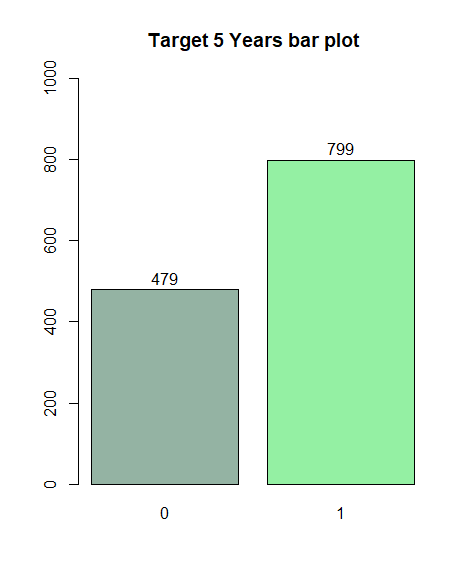
\includegraphics[width=0.5\linewidth]{ImageFiles/Classification/target_bar_plot}
	\caption{Target variable bar plot.}
	\label{fig:target_bar_plot}
\end{figure}

Afterwards, we removed an additional column from the dataset, namely \textit{"PTS"}, which is a linear combination of \textit{"FGM"}, \textit{"X3P\_MADE"}, and \textit{"FTM"}.

Therefore the dataset that will be used contains 1278 samples and 18 features.
